\newpage
\def\thoigian{90}%--Thời gian
\de{Đề số 2}{Chương I. Ứng dụng đạo hàm để khảo sát hàm số}


\begin{center}
	\textbf{PHẦN 1 - CÂU TRẮC NGHIỆM BỐN PHƯƠNG ÁN}
\end{center}
\Opensolutionfile{ans}[ans/ans-TN-ONTAPCHUONG1-DE2]
%Câu 1- Đơn điệu
\begin{ex}%[2D1H1-2]%[Dự án D - đợt 4 NH24-25- Hieu Hieu Minh Minh]
	Cho hàm $f(x)$ có bảng xét dấu $f'(x)$ như sau:
	\begin{center}
		
\begin{tikzpicture}
			\tkzTabInit[lgt=1.5, espcl=2, deltacl=.5]
			{$x$ /0.7, $f'(x)$ /0.7}
			{$-\infty$, $-3$, $1$, $2$, $+\infty$}
			\tkzTabLine{,+ , $0$, -, $0$, +, $0$, +, }
		\end{tikzpicture}
	\end{center}
	Hàm số đã cho đồng biến trên khoảng nào?
	\choice
	{$(-3;-1)$}
	{$(-\infty;-2)$}
	{\True $(1;+\infty)$}
	{$(0;2)$}
	\loigiai{
		Do $ f'(x) \ge 0 , \forall x \in (1;+\infty)$ nên hàm số đồng biến trên $(1;+\infty)$.
	}
\end{ex}
%Câu 2 - Đơn điệu
\begin{ex}%[2D1N1-2]%[Dự án D - đợt 4 NH24-25- Hieu Hieu Minh Minh]
	\immini[thm]{Cho hàm số $y=f(x)$ có đồ thị như hình vẽ bên. Hàm số $y=f(x)$ đồng biến trên khoảng nào sau đây?
		\choice
		{$(2;+\infty)$}
		{\True $(0;2)$}
		{$(-2;2)$}
		{$(-\infty;0)$}
	}
	{
		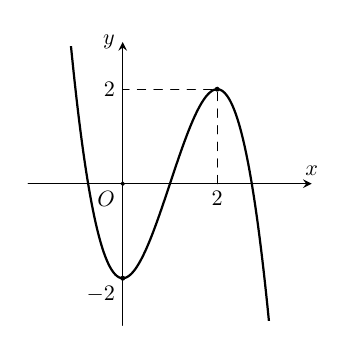
\begin{tikzpicture}[scale=0.6,>=stealth, line join=round, line cap=round]
			\def\a{-1} \def\b{3} \def\c{0} \def\d{-2} % Hệ số
			\def\xmin{-2} \def\xmax{4}
			\def\ymin{-3} \def\ymax{3} 
			%\draw[color=gray!50,dashed] (\xmin,\ymin) grid (\xmax,\ymax); 
			\draw[->] (\xmin,0)--(\xmax,0) node [above]{$x$};
			\draw[->] (0,\ymin)--(0,\ymax) node [left]{$y$};
			\draw[fill=black] (0,0) circle (1pt) node[below left]{$O$};
			\clip (\xmin+0.1,\ymin+0.1) rectangle (\xmax-0.5,\ymax-0.1);
			\draw[thick,samples=300] plot[domain=-2.5:3.5](\x,{\a*(\x)^3+\b*(\x)^2+\c*(\x)+\d});
			\draw[dashed] (2,0)|-(0,2);
			\path 
			(2,0) node[below]{$2$}
			(0,2) node[left]{$2$}
			(0,-2) node[below left]{$-2$}
			;
			\fill[black] (2,2) circle (1.5pt);
			\fill[black] (0,-2) circle (1.5pt);
		\end{tikzpicture}
	}
	\loigiai{
		Từ đồ thị của hàm số $y=f(x)$, ta thấy trên khoảng $(0;2)$ đồ thị của hàm số có hướng đi lên từ trái sang phải. \\
		Suy ra hàm số đồng biến trên khoảng $(0;2)$.
	}
\end{ex}
%Câu 3 - Cực trị
\begin{ex}%[2D1N2-1]%[Dự án D - đợt 4 NH24-25- Hieu Hieu Minh Minh]
	Cho hàm số $f(x)$ có đạo hàm là $f'(x)=x(x-1)(x+2)^2$, $\forall x \in \mathbb{R}$. Số điểm cực trị của hàm số là
	\choice
	{$5$}
	{\True $2$}
	{$1$}
	{$3$}
	\loigiai{
		Cho $f'(x)=0\Leftrightarrow \hoac{&x=0\\&x=1\\&x=-2\quad \text{(nghiệm kép).}}$\\
		Suy ra hàm số $f(x)$ có $2$ cực trị.
	}
\end{ex}
%Câu 4 - Cực trị
\begin{ex}%[2D1H2-1]%[Dự án D - đợt 4 NH24-25- Hieu Hieu Minh Minh]
	Tìm các điểm cực trị của hàm số $y=\dfrac{x^2+x+4}{x+1}$.
	\choice
	{$x_{\text{CT}}=-3$, $x_{\text{CĐ}}=1$}
	{$x_{\text{CT}}=-5$, $x_{\text{CĐ}}=3$}
	{\True $x_{\text{CĐ}}=-3$, $x_{\text{CT}}=1$}
	{$x_{\text{CĐ}}=-5$, $x_{\text{CT}}=3$}
	\loigiai{
		Xét hàm số $y=f(x)=\dfrac{x^2 + x + 4}{x + 1}$.
		\begin{enumerate}
			\item Tập xác định: $\mathscr{D}=\mathbb{R}\setminus\left\{-1\right\}$.
			\item Bảng biến thiên:\\
				Đạo hàm $y'=\dfrac{x^2 + 2 x - 3}{\left(x + 1\right)^2}$\\
				$y'=0 \Leftrightarrow x=-3$ hoặc $x=1$.
				\begin{center}
					
\begin{tikzpicture}
						\tkzTabInit[nocadre=false,lgt=1.2,espcl=2.5,deltacl=0.6]
						{$x$/0.6, $y'$/0.6, $y$/2}
						{$ -\infty $, $-3$, $-1$, $1$, $ +\infty $}
						%dòng xét dấu
						\tkzTabLine{ , +,0,-,d ,-,0, +, }
						%dòng biến thiên
						\tkzTabVar { -/$-\infty$, +/$-5$ , -D+/$-\infty$/$+\infty$, -/$3$, +/$+\infty$}
					\end{tikzpicture}
				\end{center}	
				Vậy hàm số đạt cực đại tại $x = -3$ và $y_{\text{CĐ}} = -5$.\\
				Hàm số đạt cực tiểu tại $x = 1$ và $y_{\text{CT}} = 3$.
		\end{enumerate}
	}
\end{ex}
%Câu 5 - GTNN
\begin{ex}%[2D1N3-1]%[Dự án D - đợt 4 NH24-25- Hieu Hieu Minh Minh]
	Giá trị nhỏ nhất $m$ của hàm số $y=x^3-7x^2+11x-2$ trên đoạn $[0;2]$ là
	\choice
	{$m=11$}
	{\True $m=-2$}
	{$m=3$}
	{$m=0$}
	\loigiai{
		Hàm số liên tục trên $[0;2]$.\\
		Ta có $y^{\prime}=3x^2-14x+11$.\\
		$y^{\prime}=0 \Leftrightarrow 3x^2-14x+11=0 \Leftrightarrow \hoac{&x=1\\&x=\dfrac{11}{3} \quad (\text{loại}).}$\\
		$y(0)=-2$, $y(1)=3$, $y(2)=0$.\\
		Vậy giá trị nhỏ nhất của hàm số trên đoạn $[0;2]$ là $m=-2$.
	}
\end{ex}
%Câu 6 - GTNN
\begin{ex}%[2D1B3-1]%[Dự án D - đợt 4 NH24-25- Hieu Hieu Minh Minh]
	\immini{
		Cho hàm số $y=f(x)$ liên tục trên $[-1;5]$ và có đồ thị như hình vẽ. Gọi $M$, $m$ lần lượt là giá trị lớn nhất và nhỏ nhất của hàm số $y=f(x)$ trên $[-1;5]$. Khi đó $M+m$ bằng
		\choice
		{$-1$}
		{$3$}
		{\True $1$}
		{$-2$}
	}{
		\begin{tikzpicture}[scale=0.7, font=\footnotesize, line join=round, line cap=round, >=stealth]
			\def\xmin{-2} \def\xmax{6.5}
			\def\ymin{-3} \def\ymax{4} 
			\draw[->] (\xmin,0)--(\xmax,0) node [below]{$x$};
			\draw[->] (0,\ymin)--(0,\ymax) node [left]{$y$};
			\fill (0,0)circle (1pt)node[below right]{$O$};
			\foreach \x/\g in {-1/below left,2/above, 3/below,4/below,5/below}  \draw[thin] (\x,1pt)--(\x,-1pt) node[\g]{$\x$};
			\foreach \y/\g in {-2/below right,1/left,3/left} \draw[thin] (1pt,\y)--(-1pt,\y) node[\g]{$\y$};
			\draw[dashed] (0,-2)--(2,-2)--(2,0) (0,1)--(3,1)--(3,0) 
			(0,1)--(5,1)--(5,0)
			(0,3)--(4,3)--(4,0)
			(0,-2)--(-1,-2)--(-1,0);
			\draw[red] (-1.1,-2.6) parabola bend (0,1) (1,-0.5) parabola bend (2,-2)
			(3,1) parabola bend (4,3) (5,1) 
			;
			\draw[red] (5,1)--(5.6,-2.5)
			;
			\fill[black]
			(5,1)circle(1.5pt) 
			(4,3)circle(1.5pt)
			(3,1)circle(1.5pt) 
			(0,1)circle(1.5pt)
			(2,-2)circle(1.5pt)
			(-1,-2)circle(1.5pt)
			;
		\end{tikzpicture}
	}
	\loigiai{
		Dựa vào đồ thị, giá trị lớn nhất của hàm số là $M=\max\limits_{[-1;5]} f(x)=f(4)=3$.\\
		Giá trị nhỏ nhất của hàm số là $m=\min\limits_{[-1;5]} f(x)=f(2)=f(-1)=-2$.\\
		Vậy $M+m=3-2=1$.		
	}
\end{ex}
%Câu 7 - Tiệm cận
\begin{ex}%[2D1N4-1]%[Dự án D - đợt 4 NH24-25- Hieu Hieu Minh Minh]
	Cho hàm số $y=f(x)$ xác định, liên tục trên các khoảng $(-\infty;0)$ và $(0;+\infty)$. Bảng biến thiên của hàm số $y=f(x)$ như sau:
	\begin{center}
		
\begin{tikzpicture}
			\tkzTabInit[nocadre=false,lgt=1,espcl=2.5]{$x$/0.6,$y'$/0.6,$y$/2}{$-\infty$,$0$,$3$,$+\infty$}
			\tkzTabLine{,-,d,-,$0$,+,}
			\tkzTabVar{+/ $1$,-D+ /$-\infty$  /$2$, -/$-3$, +/$3$}
		\end{tikzpicture}
	\end{center}
	Tổng số đường tiệm cận đứng và tiệm cận ngang của đồ thị hàm số đã cho là
	\choice
	{\True $3$}
	{$5$}
	{$2$}
	{$4$}
	\loigiai{
		Từ bảng biến thiên của hàm số $y=f(x)$, ta có
		\begin{itemize}
			\item $\lim\limits_{x \to -\infty}y=1$ và $\lim\limits_{x \to +\infty}y=3$ suy ra đồ thị hàm số có hai đường tiệm cận ngang $y=1$, $y=3$.
			\item $\lim\limits_{x \to 0^{-}}y=-\infty$ suy ra đồ thị hàm số có đường tiệm cận đứng $x=0$.
		\end{itemize}
		Vậy đồ thị hàm số có tổng cộng ba đường tiệm cận.
	}
\end{ex}
%Câu 8 - Tiệm cận
\begin{ex}%[2D1N4-1]%[Dự án D - đợt 4 NH24-25- Hieu Hieu Minh Minh]
	Tiệm cận ngang của đồ thị hàm số $y=\dfrac{x-2}{x+1}$ là
	\choice
	{$y=-2$}
	{\True $y=1$}
	{$x=-1$}
	{$x=2$}
	\loigiai{
		Ta có $\lim\limits_{x\to \pm\infty}y=\lim\limits_{x\to \pm\infty}\dfrac{x-2}{x+1}=\lim\limits_{x\to \pm\infty}\dfrac{1-\dfrac{2}{x}}{1+\dfrac{1}{x}}=1$ nên đường tiệm cận ngang của đồ thị hàm số là $y=1$.
		
	}
\end{ex}
%Câu 9 - Tiệm cận
\begin{ex}%[2D1H4-1]%[Dự án D - đợt 4 NH24-25- Hieu Hieu Minh Minh]
	Đường tiệm cận xiên của đồ thị hàm số $y=\dfrac{-6x^2-x+2}{2x+1}$ có phương trình là
	\choice
	{$y=3x-1$}
	{$y=-3x-1$}
	{$y=\dfrac{2}{3}x-1$}
	{\True $y=-3x+1$}
	\loigiai{
		Hàm số viết thành $y=-3x+1+\dfrac{1}{2x+1}$.\\
		Ta có $\lim\limits_{x \to \pm\infty}\left[y-(-3x+1)\right]=\lim\limits_{x \to \pm\infty}\dfrac{1}{2x+1}=0$.\\
		Suy ra $y=-3x+1$ là tiệm cận xiên của đồ thị hàm số.
	}
\end{ex}
%Câu 10 - Đồ thị
\begin{ex}%[2D1H5-1]%[Dự án D - đợt 4 NH24-25- Hieu Hieu Minh Minh]
	\immini{
		Đồ thị của hàm số nào dưới đây có dạng như đường cong trong hình bên?
		\choice
		{\True $y=x^3-3x$}
		{$y=x^3-3x^2+1$}
		{$y=-x^3+3x^2$}
		{$y=-x^3+3x$}
	}{
		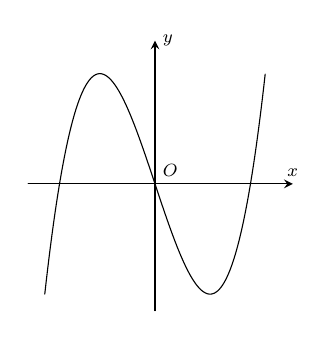
\begin{tikzpicture}[line cap=round, line join=round, font=\footnotesize,>=stealth, scale=0.7]
			\draw[->] (-2.3,0)--(2.5,0) node[above] { $x$};
			\draw[->] (0,-2.3)--(0,2.6) node[right] { $y$};
			\draw (0,0) node [above right] { $O$};
			\begin{scope}
				\clip (-2.2,-2.2) rectangle (2.5,2.5);
				\draw[samples=200,domain=-2:2,smooth] plot (\x,{1*((\x)^3)+0*((\x)^2)+-3*(\x)+0});
			\end{scope}
		\end{tikzpicture}
	}
	\loigiai{
		Dựa vào đồ thị ta thấy đây là dạng đồ thị của hàm bậc ba có hệ số $a>0$ và đi qua gốc tọa độ nên chọn đáp án là $y=x^3-3x$.
	}
\end{ex}
%Câu 11 - Đồ thị
\begin{ex}%[2D1N5-1]%[Dự án D - đợt 4 NH24-25- Hieu Hieu Minh Minh]
	\immini[thm]{
		Đường cong hình vẽ bên là đồ thị của hàm số nào trong bốn hàm số dưới đây?
		\choice
		{$y=\dfrac{2x-1}{x-1}$}
		{\True $y=\dfrac{x+1}{x-1}$}
		{$y=x^3+x^2+1$}
		{$y=x^3-3x-1$}
	}
	{
		\begin{tikzpicture}[scale=0.5, font=\footnotesize, line join=round, line cap=round, >=stealth]
			\draw[->] (-3.1,0)--(4.1,0) node[below left] {$x$};
			\draw[->] (0,-3.1)--(0,4.1) node[below left] {$y$};
%			\draw (0,0) node [above left] {$O$} circle(1pt);
			\foreach \x/\nx in {1/1}
			\draw[dashed] (\x,1pt)--(\x,-1pt) node [below left] {$\nx$};
			\foreach \y/\ny in {1/1}
			\draw[dashed] (1pt,\y)--(-1pt,\y) node [above left] {$\ny$};
			\draw[dashed] (1.01,-3)--(1.01,4);
			\begin{scope}
				\clip (-3,-3) rectangle (4,4);
				\draw[samples=200,domain=-3:0.99,smooth,variable=\x] plot (\x,{(1*(\x)+1)/(1*(\x)+-1)});
				\draw[samples=200,domain=1.01:4,smooth,variable=\x] plot (\x,{(1*(\x)+1)/(1*(\x)+-1)});
				\draw[dashed] (-3,1/1)--(4,1/1);
			\end{scope}
			\fill[black]
			(0,1)circle(1.5pt) 
			(1,0)circle(1.5pt) 
			;
		\end{tikzpicture}
	}
	\loigiai{
		Đồ thị hình bên là đồ thị hàm số dạng $y=\dfrac{ax+b}{cx+d}$.\\
		Từ đồ thị suy ra đường tiệm cận đứng là $x=1$ và đường tiệm cận ngang là $y=1$.\\
		Vậy hàm số cần tìm là $y=\dfrac{x+1}{x-1}$.
	}
\end{ex}
%Câu 12 - Đồ thị
\begin{ex}%[2D1N5-1]%[Dự án D - đợt 4 NH24-25- Hieu Hieu Minh Minh]
	\immini[thm]{
		Đường cong ở hình vẽ bên là đồ thị của hàm số nào trong bốn hàm số dưới đây?
		\choice
		{\True $y=\dfrac{-x^2-x+2}{x+1}$}
		{$y=\dfrac{-2x+1}{x+1}$}
		{$y=\dfrac{x^2+x+2}{x+1}$}
		{$y=x^3-3x^2$}
	}
	{
		\begin{tikzpicture}[scale=0.7, font=\footnotesize, line join=round, line cap=round, >=stealth]
			\draw[->] (-5.1,0)--(4.1,0) node[below left] {$x$};
			\draw[->] (0,-4.1)--(0,5.1) node[below left] {$y$};
			\draw (0,0) node [below left] {$O$} circle(1pt);
			\foreach \x/\nx in {-2/-2,-1/-1,1/1}
			\draw[thin] (\x,1pt)--(\x,-1pt) node [below left] {$\nx$};
			\foreach \y/\ny in {2/2}
			\draw[thin] (1pt,\y)--(-1pt,\y) node [left] {$\ny$};
			\draw (-0.99,-4)--(-0.99,5) node [left] {$x=-1$};
			\begin{scope}
				\clip (-5,-4) rectangle (4,5);
				\draw[samples=200,domain=-6:-1.01,smooth,variable=\x] plot (\x,{(-1*((\x)^2)+-1*(\x)+2)/(1*(\x)+1)});
				\draw[samples=200,domain=-0.99:4,smooth,variable=\x] plot (\x,{(-1*((\x)^2)+-1*(\x)+2)/(1*(\x)+1)});
				\draw (-6.1,6.1)--(4.1,-4.1) (3.2,-4) node [above left] {$y=-x$};
			\end{scope}
		\end{tikzpicture}
	}
	\loigiai{
		Đồ thị hàm số cần tìm cắt trục $Oy$ tại điểm có tung độ bằng $2$ và cắt trục $Ox$ tại hai điểm lần lượt có hoành độ bằng $-2$; $1$.\\
		Vậy hàm số có đồ thị như hình vẽ là $y=\dfrac{-x^2-x+2}{x+1}$.
	}
\end{ex}

\Closesolutionfile{ans}
%\begin{center}
%	\textbf{ĐÁP ÁN}
%	\inputansbox{10}{ans/ans}	
%\end{center}

\begin{center}
	\textbf{PHẦN 2 - CÂU TRẮC NGHIỆM ĐÚNG SAI}
\end{center}
\setcounter{ex}{0}
\Opensolutionfile{ans}[ans/answer-DS-ONTAPCHUONG1-DE2]

%Câu 1%
\begin{ex}%[2D1V4-1]%[Dự án D - đợt 4 NH24-25- Hieu Hieu Minh Minh]
	Cho hàm số $y=f(x)=\dfrac{2x-1}{x-1}$.
	\choiceTF
	{\True Tập xác định của hàm số là $\mathscr{D}=\mathbb{R}\setminus \left\{1\right\}$}
	{\True Hàm số nghịch biến trên $(-\infty;1)$ và $(1;+\infty)$}
	{\True Hàm số không có cực trị}
	{Hàm số $g(x)=f(x)+x-3$ có điểm cực đại $x=2$}
	\loigiai{
		\begin{itemchoice}
			\itemch Tập xác định $\mathscr{D}=\mathbb{R}\setminus \{1\}$.
			\itemch Ta có $y'=\dfrac{-1}{(x-1)^2} <0, \forall x \in \mathscr{D}$.\\
			Do đó hàm số nghịch biến trên $(-\infty;1)$ và $(1;+\infty)$.
			\itemch Hàm số không có cực trị.
			\itemch Ta có $g'(x)=f'(x)+1=\dfrac{-1}{(x-1)^2}+1$.\\
			Xét $g'(x)=0\Leftrightarrow \hoac{&x=2\\&x=0.}$\\
			Ta có bảng biến thiên
			\begin{center}
				
\begin{tikzpicture}[>=stealth]
					\tkzTabInit[nocadre=false,lgt=1,espcl=2,deltacl=0.5]{$x$/.6 ,$y'$/.6,$y$/2}
					{$-\infty$ , $0$ , $1$ , $2$ , $+\infty$}
					\tkzTabLine{ , + , $0$ , - , d , - , $0$ , + , }
					\tkzTabVar{-/$-\infty$ , +/$-2$ , -D+/$-\infty$/$+\infty$ , -/$2$ , +/$+\infty$}
				\end{tikzpicture}
			\end{center}
			Do đó hàm số có điểm cực đại $x=0$.
		\end{itemchoice}
	}
\end{ex}
%Câu 2%
\begin{ex}%[2D1H4-1]%[Dự án D - đợt 4 NH24-25- Hieu Hieu Minh Minh]
	Cho hàm số $y=f(x)=\dfrac{x^2-3x+1}{x-3}$ có đồ thị $(C)$.
	\choiceTF
	{\True $(C)$ có tiệm cận đứng là đường thẳng $x=3$}
	{\True $(C)$ có tiệm cận xiên là đường thẳng $y=x$}
	{$(C)$ có tâm đối xứng là điểm $I(3;4)$}
	{$\lim\limits_{x\to +\infty} y=-\infty$ và $\lim\limits_{x\to -\infty} y=+\infty$}
	\loigiai{
		Tập xác định $\mathscr{D}=\mathbb{R}\setminus\{3\}$.\\
		\begin{itemchoice}
			\itemch Ta có $\lim\limits_{x\to 3^+} f(x)=+\infty$ nên $x=3$ là tiệm cận đứng của đồ thị hàm số.
			\itemch Ta có $\lim\limits_{x\to +\infty} \left[f(x)-x\right]=0$ nên $y=x$ là tiệm cận xiên của đồ thị hàm số.
			\itemch Vì tiệm cận đứng của $(C)$ là $x=3$ và tiệm cận xiên của $(C)$ là $y=x$ nên $(C)$ có tâm đối xứng là điểm $I(3;3)$.
			\itemch $\lim\limits_{x\to +\infty} y=+\infty$ và $\lim\limits_{x\to -\infty} y=-\infty$.
		\end{itemchoice}
	}
\end{ex}
\Closesolutionfile{ans}
%\inputansbox[2]{2}{ans/answer.tex}

\begin{center}
\textbf{PHẦN 3 - CÂU TRẮC NGHIỆM TRẢ LỜI NGẮN}
\end{center}
\setcounter{ex}{0}
\Opensolutionfile{ans}[ans/ans-KQ-ONTAPCHUONG1-DE2]
%Câu 1%
\begin{ex}%[2D1H2-1]%[Dự án D - đợt 4 NH24-25- Hieu Hieu Minh Minh]
	Giả sử hàm số $f(x)=x^3 + 6x^2 + 9x +1$ đạt cực đại tại $x=a$ và đạt cực tiểu tại điểm $x=b$. Tính $P=2a+b$.
	\shortans{-7}
	\loigiai{Tập xác định $\mathscr{D}=\mathbb{R}$.\\
		Ta có $f'(x)=3x^2 + 12x +9$.\\
		Cho $f'(x)=0\Leftrightarrow \hoac{&x=-1\\ &x=-3.}$\\
		Bảng biến thiên
		\begin{center}
			
\begin{tikzpicture}
				\tkzTabInit[nocadre=false,lgt=1.2,espcl=2.5,deltacl=0.65]
				{$x$/.6,$f'(x) $/.6,$f(x)$/2}
				{$-\infty$,$-3$,$-1$,$+\infty$}
				\tkzTabLine{,+,0,-,0,+,} %
				\tkzTabVar{-/$-\infty$,+/$1$, -/$-3$,+/$+\infty$} %dấu mũi tên, + trên, -dưới
			\end{tikzpicture}
		\end{center}
		Suy ra $f(x)$ đạt cực đại tại $x=-3$ đạt cực tiểu tại $x=-1$.\\
		Suy ra $a=-3$ và $b=-1$.\\
		Vậy $P=2a+b= 2\cdot (-3) + (-1)=-7$.
	}
\end{ex}
%Câu 2%
\begin{ex}%[2D1V3-6]%[Dự án D - đợt 4 NH24-25- Hieu Hieu Minh Minh]
	Ông A muốn xây một cái bể chứa nước dạng hình hộp chữ nhật không nắp có thể tích bằng $\dfrac{500}{3}$m$^3$, đáy bể là hình chữ nhật có chiều dài gấp đôi chiều rộng. Giá thuê nhân công để xây bể là $300 \; 000$ đồng/m$^2$ (diện tích tính theo $5$ mặt trong của bể). Chi phí ông A thuê nhân công thấp nhất là bao nhiêu? (kết quả làm tròn đến đơn vị triệu đồng).
	\shortans{45}
	\loigiai{Gọi $x$ (m) là chiều rộng của cái bể chứa nước dạng hình hộp chữ nhật (với $x>0$).\\
		Theo giả thiết, chiều dài của cái bể chứa nước là $2x$ (m).\\
		Gọi $h$ (m) là chiều cao của chiếc bể. Khi đó 
		$$V= \dfrac{500}{3} \Rightarrow x \cdot 2x \cdot h =\dfrac{500}{3}  \Rightarrow h=\dfrac{250}{3x^2}.$$
		Biết giá thuê nhân công tính theo diện tích tính theo $5$ mặt trong của bể. Do đó chi phí ông A thuê nhân công để xây bể là
		$$S(x) = 300 \; 000\left(2x^2+6xh\right)= 300 \; 000 \left(2x^2+ 6x \cdot \dfrac{250}{3x^2}\right) =300 \; 000\left( 2x^2+\dfrac{500}{x} \right).$$
		Ta có $S'(x)=300 \; 000\left( 4x-\dfrac{500}{x^2} \right)$.\\
		Do đó $S'(x)= 0 \Leftrightarrow 4x-\dfrac{500}{x^2}=0 \Leftrightarrow 4x^3-500=0 \Leftrightarrow x=5$.\\
		Ta có bảng biến thiên
		\begin{center}
			
\begin{tikzpicture}
				\tkzTabInit[lgt=1.2,espcl=2.6]
				{$x$ /0.6, $S’(x)$ /0.6, $S(x)$ /2}
				{$0$,$5$,$+\infty$}
				\tkzTabLine{d,-,z,+,}
				\tkzTabVar{D+/$+\infty$,-/$S(5)$,+/$+\infty$}
			\end{tikzpicture}
		\end{center}
		Vậy giá trị nhỏ nhất của hàm số $S(x)$ trên $(0;+\infty)$ là $S(5)=45 \; 000 \; 000$ nên chi phí ông A thuê nhân công thấp nhất là $45$ (triệu đồng).
	}
\end{ex}
%Câu 3%
\begin{ex}%[2D1V3-6]%[Dự án D - đợt 4 NH24-25- Hieu Hieu Minh Minh]
	Một vật đang đứng yên thì bắt đầu chuyển động theo quy luật $s(t)=-t^3+3t^2+6t$, với $t$ (giây) là khoảng thời gian tính từ lúc vật bắt đầu chuyển động và $s$ (mét) là quãng đường vật đi được trong khoảng thời gian đó. Hỏi vật tăng tốc trong khoảng thời gian bao nhiêu giây tính từ lúc bắt đầu chuyển động?
	\shortans{1}
	\loigiai{Vận tốc của vật là $v(t)=s'(t)=-3t^2+6t+6$.\\
		Ta có $v'(t)=-6t+6$.\\
		Cho $v'(t)=0 \Leftrightarrow t=1$.\\
		Bảng biến thiên
		\begin{center}
			
\begin{tikzpicture}
				\tkzTabInit[lgt=1.2,espcl=2.5,deltacl=0.6]
				{$t$/0.6,$v'(t)$/0.6,$v(t)$/2}
				{$0$,$1$,$+\infty$}
				\tkzTabLine{,+,0,-,}
				\tkzTabVar{-/$6$,+/$9$,-/$-\infty$}
			\end{tikzpicture}
		\end{center}
		Dựa vào bảng biến thiên, ta thấy $v(t)$ tăng khi $t\in (0;1)$.\\
		Vậy vật tăng tốc trong khoảng thời gian $1$ giây tính từ lúc bắt đầu chuyển động.
	}
\end{ex}
%Câu 4%
\begin{ex}%[2D1H4-1]%[Dự án D - đợt 4 NH24-25- Hieu Hieu Minh Minh]
	Cho hàm số $y=\dfrac{3x^2-2x+6}{x+1}$ có đồ thị $(C)$. Phương trình đường tiệm cận xiên của đồ thị hàm số $(C)$ là $y=ax+b$. Biểu thức $P=a^2+b^2$ có giá trị là bao nhiêu?
	\shortans{34}
	\loigiai{
		Hàm số $y=\dfrac{3x^2-2x+6}{x+1}$ có tập xác định $\mathscr{D}=\mathbb{R}\setminus \{-1\}$.\\
		Khi đó $y=3x-5+\dfrac{11}{x+1}$.\\
		Ta có 
		\begin{itemize}
			\item $\lim\limits_{x\to +\infty}[y-(3x-5)]=\lim\limits_{x\to +\infty}\dfrac{11}{x+1}=0$.
			\item $\lim\limits_{x\to -\infty}[y-(3x-5)]=\lim\limits_{x\to -\infty}\dfrac{11}{x+1}=0$.
		\end{itemize}
		Do đó phương trình đường tiệm cận xiên là $y=3x-5$, suy ra $a=3$, $b=-5$.\\Vậy $P=a^2+b^2=9+25=34$.	
	}
\end{ex}
\Closesolutionfile{ans}


\begin{center}
	\textbf{PHẦN 4 - TỰ LUẬN}
\end{center}
\setcounter{ex}{0}
%Câu 1%
\begin{ex}%[2D1H1-5]%[Dự án D - đợt 4 NH24-25- Hieu Hieu Minh Minh]
	Cho hàm số $y = mx^3 + mx^2 + (m+1)x - 3$. Số các giá trị nguyên của tham số $m$ trong đoạn $[-100;100]$ để hàm số đã cho nghịch biến trên $\mathbb{R}$ là bao nhiêu?
	\loigiai{
		\textbf{Trường hợp 1:} Với $m = 0$, ta có $y = x - 3$ là hàm số đồng biến trên $\mathbb{R}$.\\
		$\Rightarrow m = 0$ không thỏa mãn. \\ 		
		\textbf{Trường hợp 2:} Với $m \neq 0$, ta có $y' = 3mx^2 + 2mx + m + 1$.\\
		Hàm số nghịch biến trên $\mathbb{R} \Leftrightarrow y' \leq 0, \, \forall x \in \mathbb{R}$. Khi đó \allowdisplaybreaks
		\begin{eqnarray*}
			&&\heva{&a = 3m < 0\\
				&\Delta' = m^2 - 3m(m + 1) \leq 0}\Leftrightarrow\heva{&m < 0\\
				&-2m^2 - 3m \leq 0}\\
				&\Leftrightarrow & \heva{&m < 0\\
				&\hoac{&m\leq-\dfrac{3}{2}\\&m\ge 0&}}\Leftrightarrow  m \leq -\dfrac{3}{2}.
		\end{eqnarray*}
		Kết hợp với $m \in \mathbb{Z}$ và $m \in [-100; 100]$, suy ra có tất cả $99$ giá trị $m$ thỏa mãn. 
	}
\end{ex} 
%Câu 2%
\begin{ex}%[2D1H3-6]%[Dự án D - đợt 4 NH24-25- Hieu Hieu Minh Minh]
	Một nhà phân tích thị trường làm việc cho một công ty sản xuất thiết bị gia dụng nhận thấy rằng nếu công ty sản xuất và bán $x$, ($x\ge0$) chiếc máy xay sinh tố hằng tháng thì lợi nhuận thu được (nghìn đồng) là $P(x) = -0{,}3x^3 + 36x^2 + 1\,800x - 48\,000$. Để đạt lợi nhuận lớn nhất thì công ty cần sản xuất bao nhiêu chiếc máy xay sinh tố mỗi tháng?
	\loigiai{
		Xét hàm số $P(x) = -0{,}3x^3 + 36x^2 + 1\,800x - 48\,000$, khi đó $P'(x)=-0{,}9x^2+72x^2+1\,800$.\\
		Ta có $P'(x)=0\Leftrightarrow -0{,}9x^2+72x+1\,800=0 \Leftrightarrow \hoac{&x=-20\quad(\text{loại})\\&x=100\quad(\text{thỏa mãn}).}$\\
		Ta có bảng biến thiên
		\begin{center}
			
\begin{tikzpicture}
				\tkzTabInit[nocadre=false,lgt=1.2,espcl=3,deltacl=.55]
				{$x$/0.6, $y'$/0.6, $y$/2}
				{$0$,$100$,$+\infty$}
				\tkzTabLine{,+,$0$,-,}
				\tkzTabVar{-/,+/$192\,000$,-/}	
			\end{tikzpicture}
		\end{center}
		Vậy để đạt lợi nhuận lớn nhất thì công ty cần sản xuất $100$ chiếc máy xay sinh tố.
	}
\end{ex}
%Câu 3%
\begin{ex}%[2D1V5-1]%[Dự án D - đợt 4 NH24-25- Hieu Hieu Minh Minh]
	Trong $8$ phút đầu tiên kể từ khi xuất phát, độ cao $h$ (tính bằng mét) của khinh khí cầu vào thời điểm $t$ phút được cho bởi công thức $h(t)=at^3+bt^2+ct+d\, (a\neq 0)$. Đồ thị của hàm số $h(t)$ được biểu diễn trong hình bên dưới. Tìm độ cao của khinh khí cầu vào thời điểm $5$ phút (đơn vị: mét).
	\begin{center}
		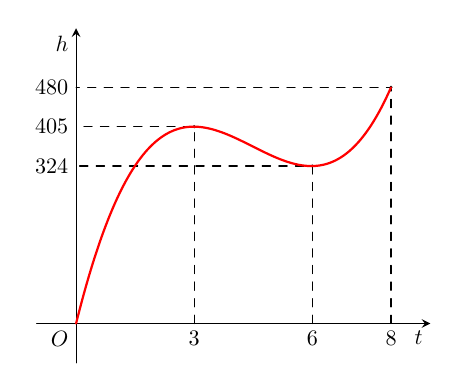
\begin{tikzpicture}[line cap=round,>=stealth,scale=0.5]
					\tikzset{every node/.style={scale=0.8}}
			\draw[->] (-1,0)--(9,0) node[below left] {$t$};
			\draw[->] (0,-1)--(0,7.5) node[below left] {$h$};
			\draw (0,0) node [below left] {$O$};
			\draw[dashed](3,0)--(3,5)--(0,5) (6,0)--(6,4)--(0,4) (8,0)--(8,6)--(0,6);
			\foreach \x in {3,6,8}{\draw (\x,0) node[below]{$\x$};}
			\draw (0,4) node[left]{$324$};
			\draw (0,5) node[left]{$405$};
			\draw (0,6) node[left]{$480$};
			\fill (3,5) circle (1.2pt);
			\fill (6,4) circle (1.2pt);
			\fill (8,6) circle (1.2pt);
			\begin{scope}
				\clip (-1,-1) rectangle (9,7);
				\draw[samples=200,domain=0:8,smooth,variable=\x,thick,red] plot (\x,{(3/40)*(\x)^3-(121/120)*(\x)^2+(241/60)*(\x)});
			\end{scope}
		\end{tikzpicture}
	\end{center}
	\loigiai{
		Gọi $(C)$ là đồ thị hàm số. Ta có
		$O(0;0)\in (C)\Leftrightarrow d=0$.\\
		$A(3;405)\in (C)\Leftrightarrow 405=27a+9b+3c$;\\
		$B(6;324)\in (C)\Leftrightarrow 324=216a+36b+6c$;\\
		$C(8;480)\in (C)\Leftrightarrow 480=512a+64b+8c$.\\
		Ta có hệ phương trình
		\[
		\heva{&27a+9b+3c=405\\
			&216a+36b+6c=324\\
			&512a+64b+8c=480}
		\Leftrightarrow
		\heva{&a=6\\&b=-81\\&c=324.}
		\]
		Do đó, ta có $h(t)=6t^3-81t^2+324t$.\\
		Tại thời điểm $t=5$ phút, ta có $h(5)=345$ mét.
	}
\end{ex}